\documentclass[a4paper, 12pt]{article}
\usepackage[left=2cm, right=2cm, top=2cm, bottom=2cm]{geometry}
\setlength{\parindent}{0cm}
\usepackage{graphicx}
\usepackage{caption}
\usepackage{color}
\begin{document}


\begin{figure}[h]
\centering

\includegraphics[width=1\textwidth]{iitm.png}
\caption{\textit{\color{red}{Indian Institute of Technology, Madras}}}
\label{image-IIT Madras}
\end{figure}

 \title{\color{red}{{\huge ID2090 : Introduction to Scientific Computing}}}

\author{Dhaval Raghwani \\ BE19B027}

\date{\today}
\maketitle

{\color{blue}\tableofcontents}

\listoffigures

\listoftables

\section{Introduction}
\texttt{This is my first course in Scientific computing.It was an eye-opening course and blessed to learn this course under the guidance of the Proffesor {\color{blue}\textit{Dr.Gandham Phanikumar!}}}
% Here is some comment that will serve documentation purpose but not get included in the 
% final output



Here is an example of an inline equation showing $\alpha = \beta + \gamma^2$.

In this document we have equation~\ref{eqn:phin} talking about how summation is represented. Also, we have equation~\ref{eqn:zetax} showing how integration is represented~\cite{dewar}. 

In this document we have table~\ref{tab:1} which is the first table we entered in the document.
We inserted one more table~\ref{tab:2} in this document just to check automatic numbering~\cite{bern}.

\begin{equation}
 \phi_n = \sum_{n=0}^{n=\infty}{ \Omega_n}
	\label{eqn:phin}
\end{equation}

Let us see if inline equation looks fine 

\begin{equation}
\zeta_x = \int_{n=0}^{n=x}{\omega_n dn}  
\label{eqn:zetax}
\end{equation}

\section{Analysis}

\begin{enumerate}
	\item First item
		\begin{enumerate}
			\item First sub item
			\item Second sub item
		\end{enumerate}
	\item Second item
\end{enumerate}

\begin{figure}[h]
	\begin{center}
		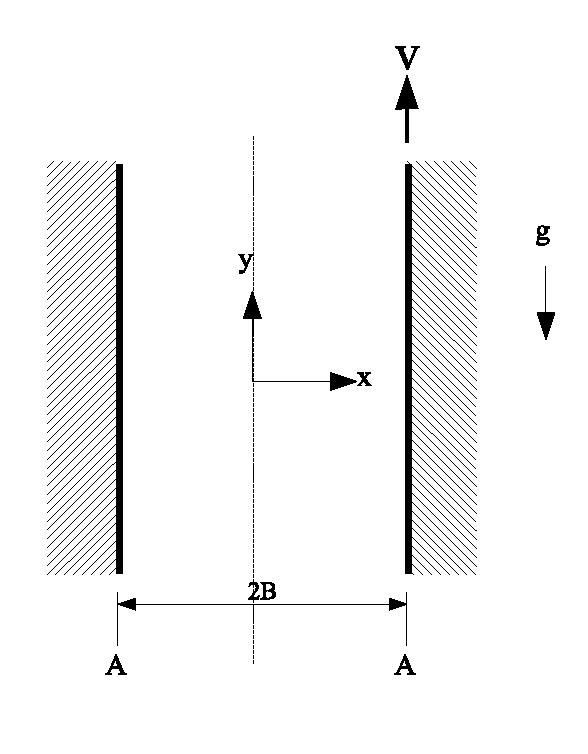
\includegraphics[scale=0.5]{schematic1.eps}
	\end{center}
	\caption{The second image we inserted in the document}
	\label{f2}
\end{figure}


\begin{figure}[h]
	\begin{center}
		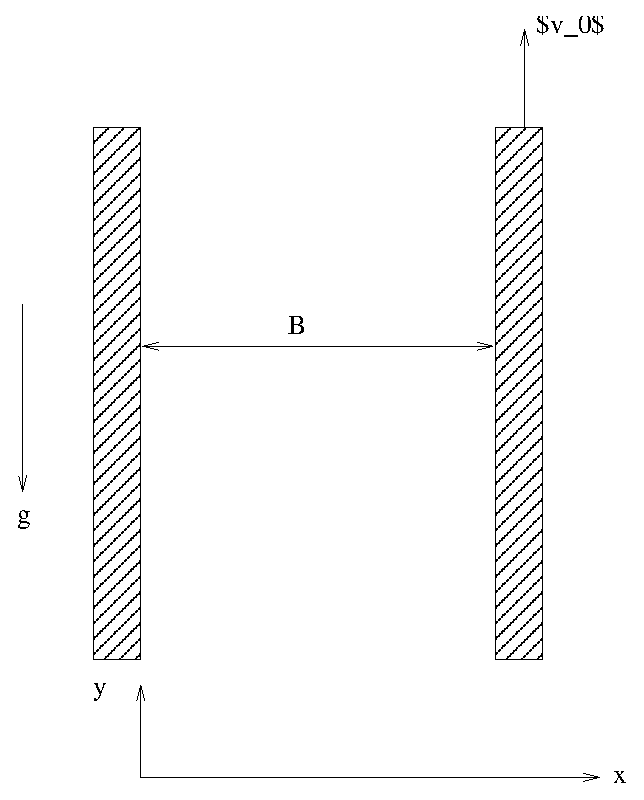
\includegraphics[scale=0.5]{fig1.eps}
	\end{center}
	\caption{Flow of liquid between two vertical plates}
	\label{f1:plates}
\end{figure}



\subsection{More analysis}
This is an example for a very long line which may or may not fit in a single line but let us see if it will wrap up in the final output rendered by latex. In figure~\ref{f1:plates} we can see the domain for the problem of flow between two vertical plates. The arrows indicate vectors for the body force terms.In figure~\ref{f2} we have inserted one more image.

\begin{table}
	\begin{center}
\begin{tabular}{|l|l|}
	\hline
	header-1 & header-2 \\
	\hline
	row-1-col-1 & row-1-col-2 \\
	row-2-col-1 & row-2-col-2 \\
	\hline
\end{tabular}
	\caption{The second table I entered in the document}
	\label{tab:2}
	\end{center}
\end{table}


\subsubsection{A minor point}
You can have only a depth of sub-sub-section in article environment but that suffices for articles.


\section{Conclusions}

\begin{itemize}
	\item One item
	\item Another item
	\item Yet another item
\end{itemize}

\begin{table}
	\begin{center}
\begin{tabular}{|l|l|}
	\hline
	row-1-col-1 & row-1-col-2 \\
	\hline
	row-2-col-1 & row-2-col-2 \\
	row-3-col-1 & row-3-col-2 \\
	row-4-col-1 & row-4-col-2 \\
	\hline
\end{tabular}
	\caption{The first table I entered in the document}
	\label{tab:1}
	\end{center}
\end{table}

\vspace{56pt}

\bibliography{mfdocrefs}
\bibliographystyle{apalike}

\end{document}
